\documentclass[border=10pt]{standalone}
\usepackage{tikz}
\usetikzlibrary{er, positioning, fit, calc, shapes.geometric}

\begin{document}

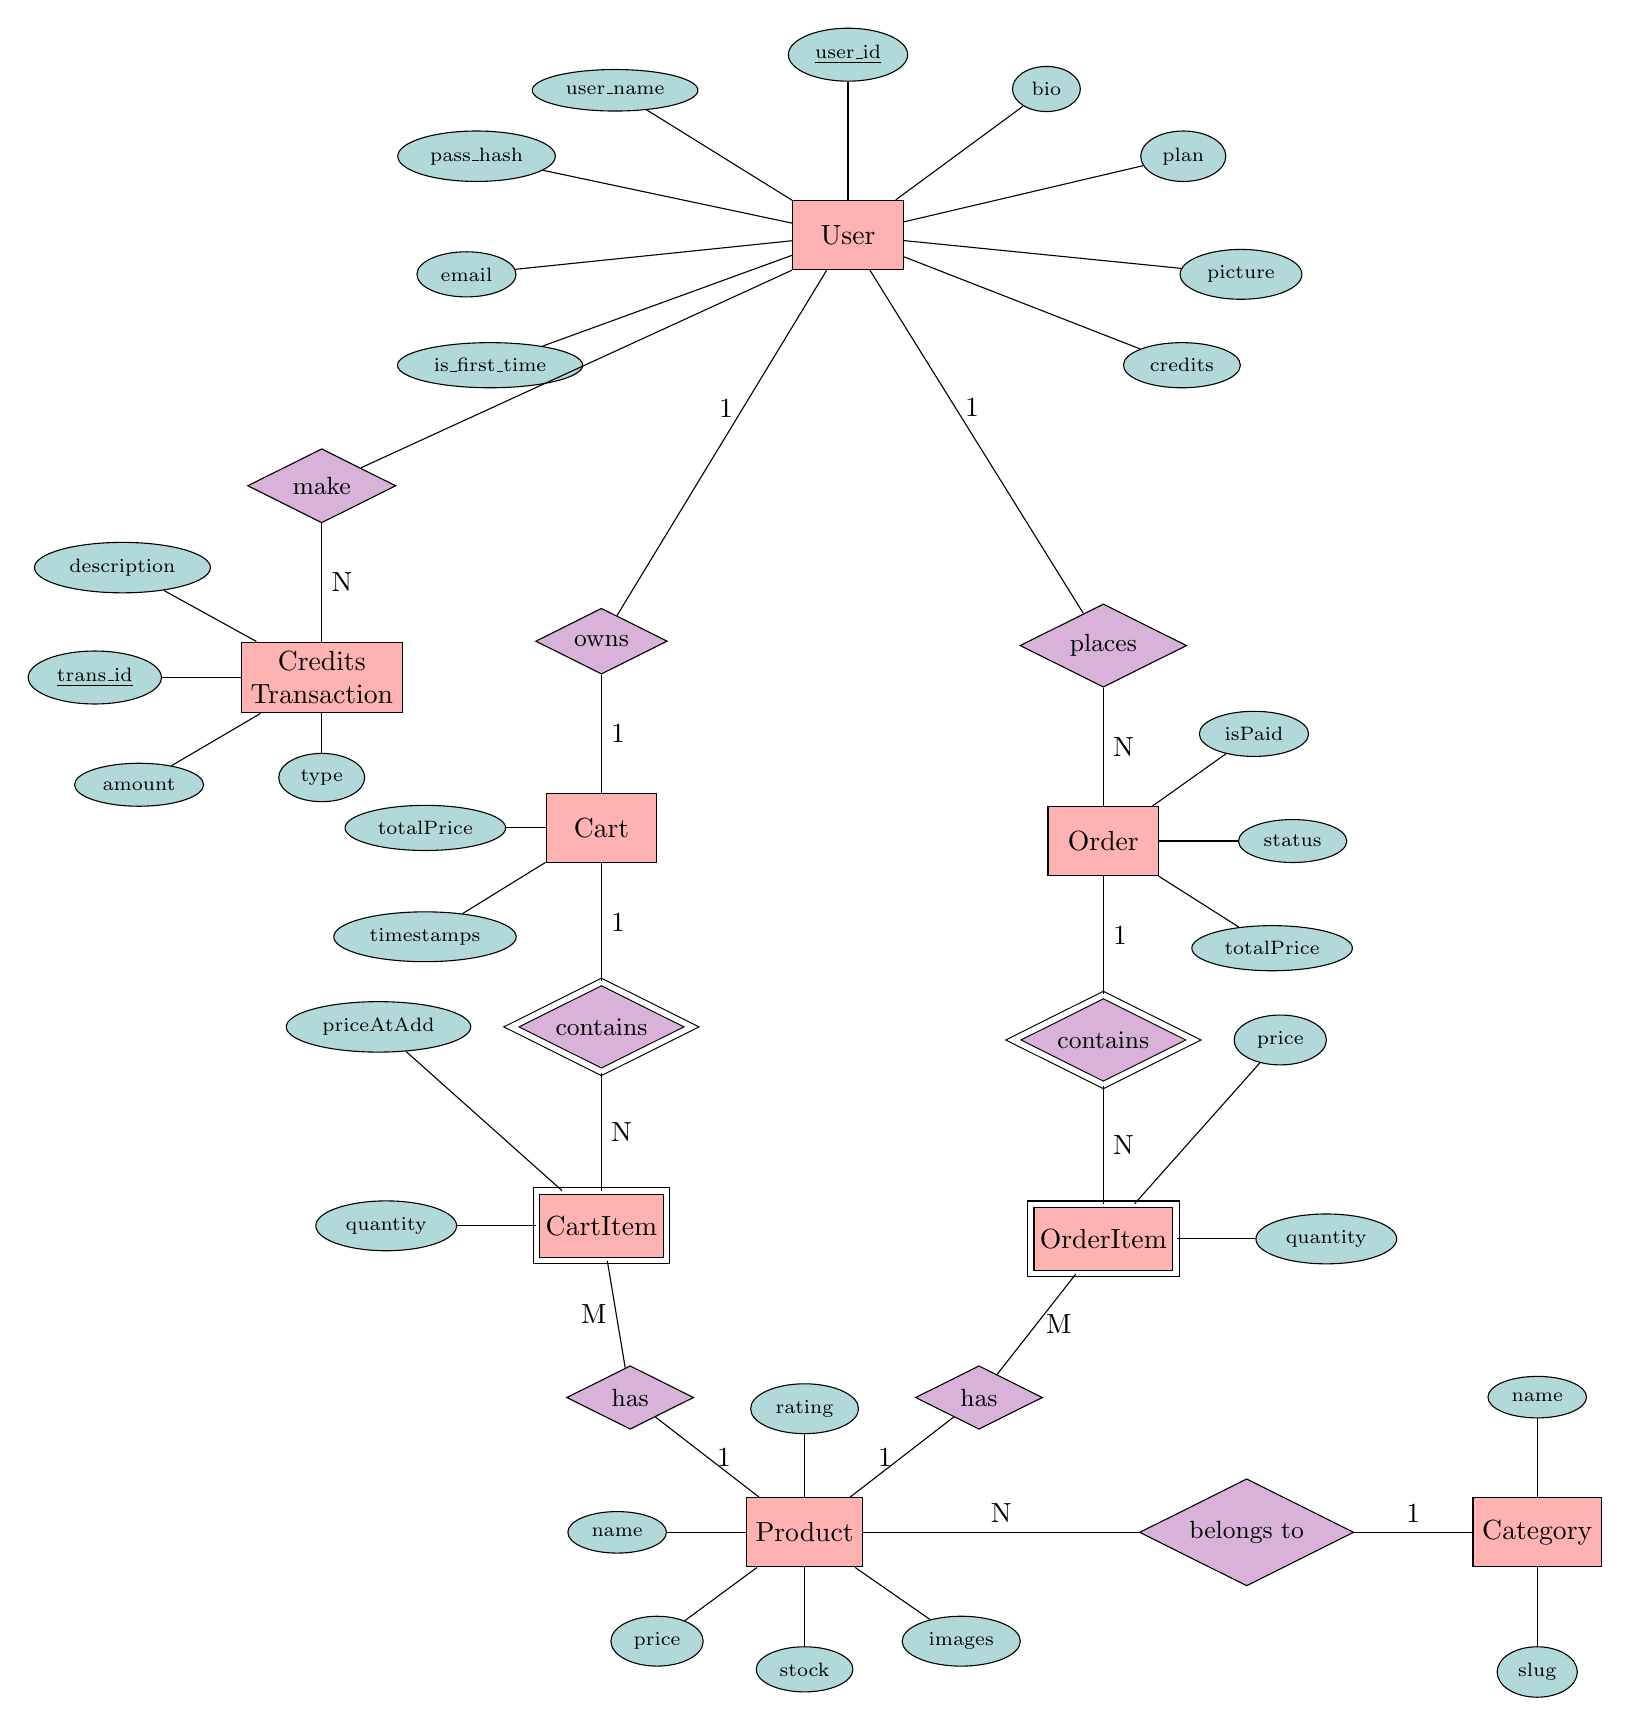
\begin{tikzpicture}[
    node distance=2cm,
    entity/.style={
        draw, 
        rectangle, 
        fill=red!30, 
        minimum height=2.5em, 
        minimum width=4em, 
        align=center
    },
    weak entity/.style={
        entity,
        double,
        double distance=2pt
    },
    attribute/.style={
        draw, 
        ellipse, 
        fill=teal!30, 
        minimum height=1.5em, 
        align=center,
        font=\scriptsize
    },
    relationship/.style={
        draw, 
        diamond, 
        fill=violet!30, 
        aspect=2, 
        minimum height=1.5em, 
        align=center,
        font=\small
    },
    weak relationship/.style={
        relationship,
        double,
        double distance=2pt
    },
    every edge/.style={
        draw, 
        thick
    }
]

    % ---------------------------------------------------------
    % 1. USER (Top Center) - FIXED SPACING
    % ---------------------------------------------------------
    \node[entity] (user) {User};
    
    % Top Vertical
    \node[attribute] (uid) [above=1.5cm of user] {\underline{user\_id}};
    
    % Top Left Fan (Spread out)
    \node[attribute] (uname) [above left=1.2cm and 1.5cm of user] {user\_name};
    \node[attribute] (pass) [left=3cm of user, yshift=1cm] {pass\_hash}; 
    
    % Bottom Left Fan
    \node[attribute] (email) [left=3.5cm of user, yshift=-0.5cm] {email};
    \node[attribute] (first) [below left=1cm and 3cm of user] {is\_first\_time};

    % Top Right Fan
    \node[attribute] (bio) [above right=1.2cm and 1.5cm of user] {bio};
    \node[attribute] (plan) [right=3cm of user, yshift=1cm] {plan};
    
    % Bottom Right Fan
    \node[attribute] (pic) [right=3.5cm of user, yshift=-0.5cm] {picture};
    \node[attribute] (cred) [below right=1cm and 3cm of user] {credits};

    % Connections
    \draw (user) -- (uid);
    \draw (user) -- (uname);
    \draw (user) -- (pass);
    \draw (user) -- (email);
    \draw (user) -- (first);
    \draw (user) -- (bio);
    \draw (user) -- (plan);
    \draw (user) -- (pic);
    \draw (user) -- (cred);

    % ---------------------------------------------------------
    % 2. CREDITS (Far Left)
    % ---------------------------------------------------------
    % Pushed further down/left to avoid the new User attributes
    \node[relationship] (make_trans) [below left=2.5cm and 5.5cm of user] {make};
    \node[entity] (trans) [below=1.5cm of make_trans] {Credits\\Transaction};
    
    \node[attribute] (tid) [left=1cm of trans] {\underline{trans\_id}};
    \node[attribute] (amt) [below left=1cm of trans] {amount};
    \node[attribute] (type) [below=0.5cm of trans] {type};
    \node[attribute] (desc) [above left=1cm of trans] {description}; 

    % Connect User -> Make (Start line from bottom-left corner of user to avoid attributes)
    \draw (user.south west) -- (make_trans); 
    \draw (make_trans) -- node[right]{N} (trans);
    \draw (trans) -- (tid);
    \draw (trans) -- (amt);
    \draw (trans) -- (type);
    \draw (trans) -- (desc);

    % ---------------------------------------------------------
    % 3. CART BRANCH (Mid Left)
    % ---------------------------------------------------------
    % Adjusted positioning to clear User attributes
    \node[relationship] (owns_cart) [below left=4.5cm and 2cm of user] {owns};
    \node[entity] (cart) [below=1.5cm of owns_cart] {Cart};
    
    \node[attribute] (ctotal) [left=0.5cm of cart] {totalPrice};
    \node[attribute] (ctime) [below left=1cm of cart] {timestamps};
    \draw (cart) -- (ctotal);
    \draw (cart) -- (ctime);

    % Cart Item
    \node[weak relationship] (contains_item) [below=1.5cm of cart] {contains};
    \node[weak entity] (cartitem) [below=1.5cm of contains_item] {CartItem};
    
    \node[attribute] (ci_qty) [left=1cm of cartitem] {quantity};
    \node[attribute] (ci_price) [left=0.5cm of contains_item] {priceAtAdd};
    \draw (cartitem) -- (ci_qty);
    \draw (cartitem) -- (ci_price);

    % Connect User -> Cart
    \draw (user) -- node[left, pos=0.4]{1} (owns_cart);
    \draw (owns_cart) -- node[right]{1} (cart);
    \draw (cart) -- node[right]{1} (contains_item);
    \draw (contains_item) -- node[right]{N} (cartitem);

    % ---------------------------------------------------------
    % 4. ORDER BRANCH (Mid Right)
    % ---------------------------------------------------------
    \node[relationship] (owns_order) [below right=4.5cm and 2cm of user] {places};
    \node[entity] (order) [below=1.5cm of owns_order] {Order};

    \node[attribute] (ostatus) [right=1cm of order] {status};
    \node[attribute] (oispaid) [above right=1cm of order] {isPaid};
    \node[attribute] (ototal) [below right=1cm of order] {totalPrice};
    \draw (order) -- (ostatus);
    \draw (order) -- (oispaid);
    \draw (order) -- (ototal);

    % Order Item
    \node[weak relationship] (ord_contains) [below=1.5cm of order] {contains};
    \node[weak entity] (orderitem) [below=1.5cm of ord_contains] {OrderItem};

    \node[attribute] (oi_qty) [right=1cm of orderitem] {quantity};
    \node[attribute] (oi_price) [right=0.5cm of ord_contains] {price};
    \draw (orderitem) -- (oi_qty);
    \draw (orderitem) -- (oi_price);

    % Connect User -> Order
    \draw (user) -- node[right, pos=0.4]{1} (owns_order);
    \draw (owns_order) -- node[right]{N} (order);
    \draw (order) -- node[right]{1} (ord_contains);
    \draw (ord_contains) -- node[right]{N} (orderitem);

    % ---------------------------------------------------------
    % 5. PRODUCT (Bottom Center)
    % ---------------------------------------------------------
    \node[entity] (product) [below right=3cm and 1cm of cartitem] {Product};

    \node[relationship] (has_prod_1) [above left=1.5cm of product] {has};
    \node[relationship] (has_prod_2) [above right=1.5cm of product] {has};

    \draw (cartitem) -- node[left]{M} (has_prod_1);
    \draw (has_prod_1) -- node[right]{1} (product);
    \draw (orderitem) -- node[right]{M} (has_prod_2);
    \draw (has_prod_2) -- node[left]{1} (product);

    \node[attribute] (pname) [left=1cm of product] {name};
    \node[attribute] (pprice) [below left=1cm of product] {price};
    \node[attribute] (pstock) [below=1cm of product] {stock};
    \node[attribute] (pimg) [below right=1cm of product] {images};
    \node[attribute] (prate) [above=0.8cm of product] {rating}; 
    
    \draw (product) -- (pname);
    \draw (product) -- (pprice);
    \draw (product) -- (pstock);
    \draw (product) -- (pimg);
    \draw (product) -- (prate);

    % ---------------------------------------------------------
    % 6. CATEGORY (Far Right)
    % ---------------------------------------------------------
    \node[relationship] (belongs) [right=3.5cm of product] {belongs to};
    \node[entity] (category) [right=1.5cm of belongs] {Category};

    \node[attribute] (cname) [above=1cm of category] {name};
    \node[attribute] (cslug) [below=1cm of category] {slug};

    \draw (product) -- node[above]{N} (belongs);
    \draw (belongs) -- node[above]{1} (category);
    \draw (category) -- (cname);
    \draw (category) -- (cslug);

\end{tikzpicture}

\end{document}